%% Ejemplo de la plantilla de latex para las diapositivas del Máster en IA 

%%%%%%%%%%%%%%%%%%%%%%%%%%%%
%% Valores para el ratio de aspecto: 43, 169 
\documentclass[10pt, envcountsect, presentation, aspectratio=169]{beamer}
%%%%%%%%%%%%%%%%%%%%%%%%%%%%

%%%%%%%%%%%%%%%%%%%%%%%%%%%%
%% Incluir fichero de estilo del máster
\input plantillaTAREA.sty
%%%%%%%%%%%%%%%%%%%%%%%%%%%%

\let\Tiny=\tiny
%\usepackage[latin1]{inputenc}
\usepackage[utf8]{inputenc}
\usepackage[spanish]{babel}
\usepackage{pgf}
\usepackage{latexsym}
\usepackage{amssymb,amsmath}
\usepackage{xspace}
\usepackage[olditem,oldenum]{paralist}
\usepackage{tikz}
\usetikzlibrary{snakes,arrows,shapes}
\usetikzlibrary{positioning}
\usetikzlibrary{arrows,automata}
\usepackage[T1]{fontenc}
\usepackage{psfrag}
\usepackage{multirow}
\usepackage{xmpmulti}
\usepackage[absolute, overlay]{textpos}
\usepackage{pgfpages}
\usepackage{pgf}
\usepackage{colortbl}
\usepackage{xcolor}
\usepackage{color}

%%%%%%%%%%%%%%%%%%%%%%%%%%%%
%% Información que aparecerá en la portada
\title[Nombre]{Modelos de Computación}
\subtitle{Entrega de Complejidad} % short title for footer

\author[Carrillo G., Gallego J., Ibarrola Y.] % Para el pie de página, poner los autores abreviados separados por comas.
{
	\sc{Ginés Carrillo Ibáñez}\\  % Autor 1
	\textit{Grupo 1. Subgrupo 9}\\
	\sc{Juan Diego Gallego Nicolás}\\ % Autor 2
	\textit{Grupo 1. Subgrupo 9}\\ 
	\sc{Yago Ibarrola Lapeña}\\ % Autor 3
	\textit{Grupo 1. Subgrupo 9}\\ 
}

\institute[GII]% % Poner las iniciales de los diferentes departamentos de los autores separadas por comas.
{
	\textit{Universidad de Murcia}
}

\date{2024/2025} % Curso académico

%%%%%%%%%%%%%%%%%%%%%%%%%%%%%%%%%%
%% Contenido de las diapositivas
\setbeamerfont{normal text}{size=\normalsize} % Modifica el tamaño del texto de las diapositivas.
\AtBeginDocument{\usebeamerfont{normal text}}

%%%%%%%%%%%%%%%%%%%%%%%%%%%%%%%%%%

\newcommand{\ldfa}{\ensuremath{\mathcal L_{DFA}}}
\newcommand{\lnfa}{\ensuremath{\mathcal L_{NFA}}}
\newcommand{\ler}{\ensuremath{\mathcal L_{ER}}}
\newcommand{\lreg}{\ensuremath{\mathcal {REG}}}
\newcommand{\lcf}{\ensuremath{\mathcal CF}}
\newcommand{\lpda}{\ensuremath{\mathcal L_{PDA}}}
\newcommand{\lpdav}{\ensuremath{\mathcal L_{PDA^v}}}
\newcommand{\lpdad}{\ensuremath{\mathcal L_{PDAD}}}
\newcommand{\lgr}{\ensuremath{\mathcal L_{GCF}}}
\newcommand{\ld}{\ensuremath{\mathcal {DEC}}}
\newcommand{\lr}{\ensuremath{\mathcal {RE}}}
\newcommand{\halt}{\ensuremath{\mathsf{HALT}}}
\newcommand{\fon}{\ensuremath{FO(\mathbb N)}}
\newcommand{\pol}{\ensuremath{\mathcal P}}
\newcommand{\npol}{\ensuremath{\mathcal{NP}}}
\newcommand{\cnpol}{\ensuremath{\mathcal{CO-NP}}}
\newcommand{\cnlo}{\ensuremath{\mathcal{CO-NLOG}}}
\newcommand{\cnpols}{\ensuremath{\mathcal{CO-NPSPACE}}}
\newcommand{\fo}{\ensuremath{FO}}
\newcommand{\lop}{\ensuremath{LP}}
\newcommand{\cnf}{\ensuremath{_{cnf}}}
\newcommand{\tcnf}{\ensuremath{_{3cnf}}}
%\newcommand{\cnf}{\ensuremath{LP_{cnf}}}
%\newcommand{\tcnf}{\ensuremath{LP_{3cnf}}}
\newcommand{\qlop}{\ensuremath{QLP}}
\newcommand{\dcnf}{\ensuremath{LP_{2cnf}}}
\newcommand{\pols}{\ensuremath{\mathcal{PSPACE}}}
\newcommand{\npols}{\ensuremath{\mathcal{NPSPACE}}}
\newcommand{\lo}{\ensuremath{\mathcal{LOG}}}
\newcommand{\nlo}{\ensuremath{\mathcal{NLOG}}}
\newcommand{\ext}{\ensuremath{\mathcal{EXPTIME}}}
\newcommand{\extn}{\ensuremath{\mathcal{NEXPTIME}}}
\newcommand{\exts}{\ensuremath{\mathcal{EXPSPACE}}}
\newcommand{\ej}{{\color{green}ejemplo}}
\newcommand{\usigma}{\ensuremath{\mathcal U}_{\Sigma}}
\newcommand{\mt}{\ensuremath{\mathcal {MT}}} 
\newcommand{\pnp}{¿\ensuremath{\mathcal{P}=\mathcal{NP}}? }

%%%%%%%%%%%%%%%%%%%%%%%%%%%%%%%%%%

\begin{document}	

%%%%%%%%%%%%%%%%%%%%%%%%%%%%%%%%%%

%%%%%%%%%%%%%%%%%%%%%%%%%%%%%%%%%%

\begin{frame}[plain]
	\titlepage
\end{frame}

%%%%%%%%%%%%%%%%%%%%%%%%%%%%%%%%%%

\begin{frame}{Problema Decisional de la Clique en un Grafo No Dirigido}{$k-clique$}
    % \vskip -1cm % Para subir (-) o bajar el texto
    \textbf{Definición:} dado un grafo no dirigido $G=(V,E)$ y un entero positivo $k$, un $k-clique$ es un subgrafo de $G$ que es completo. $G'=(V',E') \subseteq (V,E)$ es $k-clique$ de $G \Leftrightarrow \frac{|V'|(|V'|-1)}{2} \Leftrightarrow$ $\forall v, w \in V', v \neq w \text{ } (v,w)\in E'$. Un $k-clique$ también puede recibir el nombre de $clique$ de orden $k$. \\~\\

    \textbf{Propiedades:}

    \begin{itemize}
        \item[] Todo grafo no vacío tiene al menos un $1-clique$
        \item[] Todo grafo $G=(V,E)$ con $E \neq \emptyset$ tiene al menos un $2-clique$
        \item[] Si un grafo tiene un $k-clique$, tiene $cliques$ de todos los órdenes de $1$ 
        \item[] Todo grafo completo de $n$ vértices tiene $cliques$ de todos los órdenes de $1$ a $n$
    \end{itemize}
    
\end{frame}

\begin{frame}{Problema Decisional de la Clique en un Grafo No Dirigido}{$k-clique$}
    % \vskip -1cm % Para subir (-) o bajar el texto
    En el siguiente grafo podemos encontrar cliques de órdenes de $1$ hasta $4$:
    \begin{figure}
        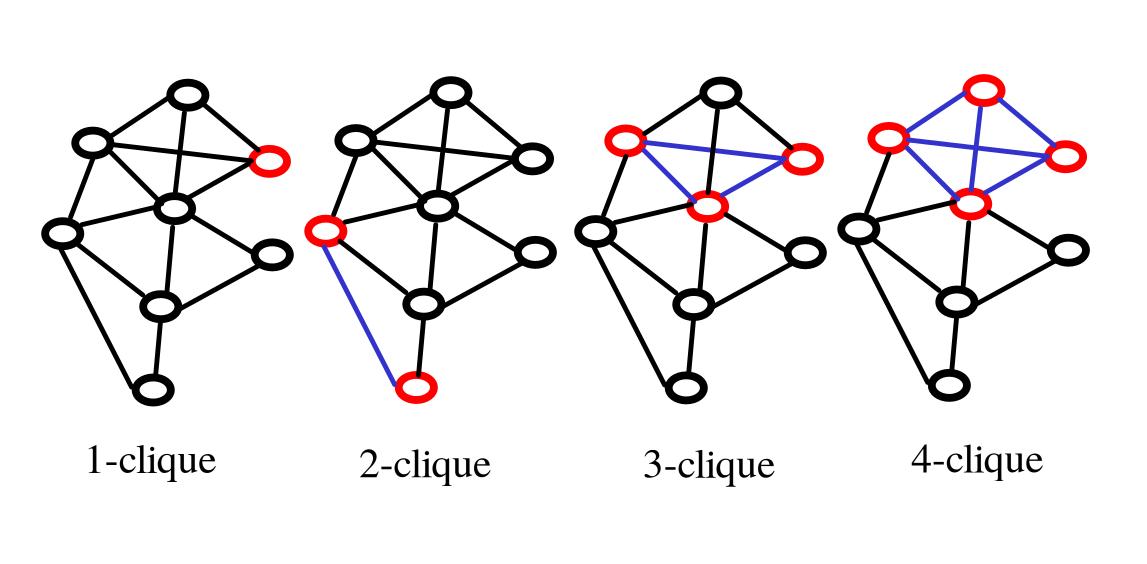
\includegraphics[scale=0.25]{images/T2_2_ejemploclique.png}
    \end{figure} 
\end{frame}

\begin{frame}{Problema Decisional de la Clique en un Grafo No Dirigido}{El lenguaje $K-CLIQUE$}
    % \vskip -1cm % Para subir (-) o bajar el texto
    \textbf{Definición:} se define el lenguaje $K-CLIQUE$ como:
    $$
    K-CLIQUE:=\{\langle G \rangle \mid G \text{ es un g.n.d. con un } K-clique\}
    $$

    \textbf{Proposición:} $K-CLIQUE \in \mathcal{P} \text{  } \forall K>0$ \\
    \textbf{Demostración:} basta diseñar una $MT$ que compruebe las $\binom{|V|}{k} = \frac{|V|!}{k!(|V|-k)!}=O(|V|^k)$ posibles combinaciones sin repetición de nodos del grafo codificado. Sea $M_K$ la $MT$ que ante una entrada $\langle G \rangle$:
    \begin{enumerate}[I]
        \item Decodifica la entrada
        \item Si $|V|<K$ RECHAZA
        \item Para cada subconjunto $V_K\subseteq V$ de $K$ vértices de $G=(V,E)$ comprobar si existe una arista en $E$ para cada par de vértices distintos de $V_K$.
        \item Si algún $V_K$ no cumple la condición RECHAZA, sino ACEPTA
    \end{enumerate}
    Como $|E|<|V|^2$, se trata de una máquina determinista con complejidad polinómica.
\end{frame}

\begin{frame}{Problema Decisional de la Clique en un Grafo No Dirigido}{El lenguaje $CLIQUE$}
    % \vskip -1cm % Para subir (-) o bajar el texto
    \textbf{Definición:} se define el lenguaje $CLIQUE$ como:
    $$
    CLIQUE:=\{\langle G, k \rangle \mid G \text{ es un g.n.d. con un } k-clique\}
    $$
    Por la diapositiva anterior, pudiera parecer que $CLIQUE \in \mathcal{P}$ trivialmente.
    No obstante, veremos más adelante que el lenguaje es $\mathcal{NP}-$completo. Primero veamos que es $\mathcal{NP}$ \\~\\

    \textbf{Proposición:} $CLIQUE \in \mathcal{NP}$

    \textbf{Demostración: } Sea $M_{CLIQUE}$ la $MT$ no determinista que ante una entrada $\langle G, k \rangle$:

    \begin{enumerate}[I]
        \item Elige un subconjunto $V_k \subseteq V$ de $k$ vértices de $G=(V,E)$
        \item Compruba que hay un arco entre cada par de vértices de $V_k$
    \end{enumerate}

    Por el mismo razonamiento que en el caso de $M_K$, $M_{CLIQUE}$ es una $MTND$.
\end{frame}

\begin{frame}{Problema Decisional de la Clique en un Grafo No Dirigido}{El lenguaje $CLIQUE$ es $\mathcal{NP}-$completo}
    Para demostrar la $\mathcal{NP}-$completitud de $CLIQUE$ vamos a necesitar las siguientes propiedades que no demostramos:
    \begin{enumerate}[1]
        \item El lenguaje $3SAT$ formado por las formulas de lógica proposicional de la forma $\bigwedge_{i=1}^n(p_1^i \vee p_2^i \vee p_3^i)$ satisfacibles es $\mathcal{NP}-$completo.
        \item \textbf{Tercer Teorema de la Reducibilidad:} sean $L$ y $L'$ dos lenguajes con $L \leq_p L'$. Si $L$ es $\mathcal{NP}-$completo y $L'$ es $\mathcal{NP}$, entonces $L'$ es $\mathcal{NP}-$completo. 
    \end{enumerate}
    Si demostramos $3SAT \leq_p CLIQUE$ tendremos el resultado que buscamos. 
\end{frame}

\begin{frame}{Problema Decisional de la Clique en un Grafo No Dirigido}{El lenguaje $CLIQUE$ es $\mathcal{NP}-$completo}
    Sea $\Phi=\bigwedge_{i=1}^n(p_1^i \vee p_2^i \vee p_3^i)$ una fórmula proposicional cualquiera. Sea $M$ la $MT$ que toma como entrada $\Phi$ y construye un grafo $G_\Phi$:
    \begin{enumerate}
        \item Para cada $i=1,\dots,n$, crea un grupo de tres vértices $V_{p_1^i}, V_{p_2^i}, V_{p_3^i}$
        \item Crea una arista entre cualquier par de véctices $V_{p_a^i}$, $V_{p_b^j}$ que cumpla:
        \begin{itemize}
            \item[] $i \neq j$
            \item[] $p_a^i \neq \neg p_b^j$ (como variables)
        \end{itemize}
    \end{enumerate}
    Es decir, crea 3 nodos por cláusula (uno por literal) y conecta cada nodo con todos los nodos de otras cláusulas con los que no haya un conflicto lógico.
    Es claro que el proceso de generación del grafo es polinomial con respecto al número de cláusulas de $\Phi$
\end{frame}

\begin{frame}{Problema Decisional de la Clique en un Grafo No Dirigido}{El lenguaje $CLIQUE$ es $\mathcal{NP}-$completo}
    Tomemos como ejemplo la fórmula de la tarea: 
    $$
    \Phi = (p_1 \vee p_2 \vee p_3) \wedge (\neg p_2 \vee p_3 \vee p_4) \wedge (p_3 \vee p_4 \vee p_5) \wedge(\neg p_4 \vee \neg p_5 \vee p_6)
    $$
    Aplicando el proceso definido en la diapositiva anterior, el grafo $G_\Phi$ es el complementario al siguiente\footnote{Es más fácil de visualizar el complementario ya que el grafo tiene muchos vértices}:
    \begin{figure}
        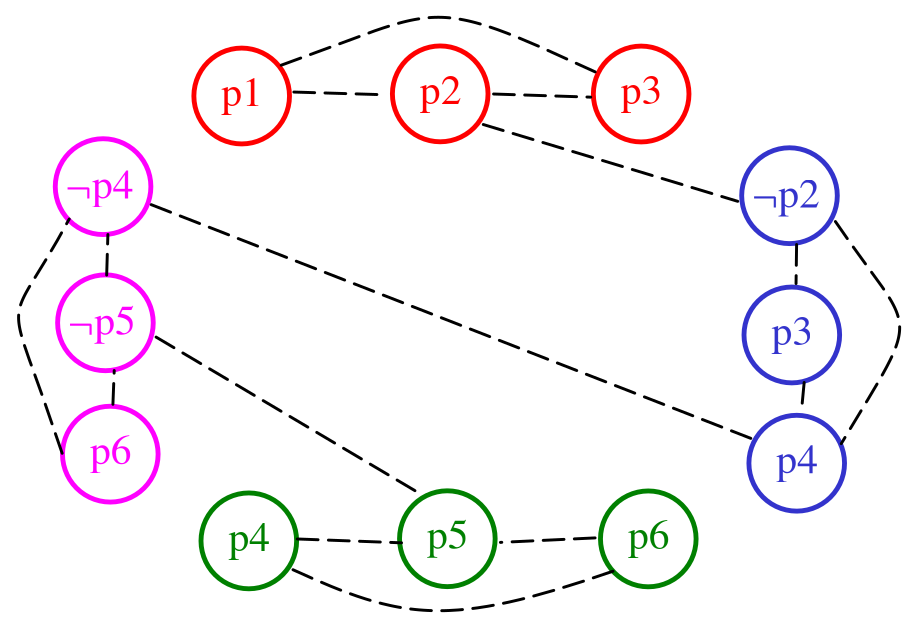
\includegraphics[scale=0.15]{images/T2_2_ejemplophi.png}
    \end{figure} 
\end{frame}

\begin{frame}{Problema Decisional de la Clique en un Grafo No Dirigido}{El lenguaje $CLIQUE$ es $\mathcal{NP}-$completo}
    \textbf{Teorema:} Dado un entero $k>0$ y $\Phi=\bigwedge_{i=1}^k(p_1^i \vee p_2^i \vee p_3^i)$ una proposición, $\Phi \in 3SAT \Leftrightarrow G_\Phi$ tiene un $k-clique$ \\~\\

    \textbf{Demostración:} \\
    $\boxed{\Rightarrow}$ Si $\Phi$ es satisfacible. Elegimos un literal $p_i^{a_i}$ para cada $i=1,\dots,k$ ($a_i=1,2,3$). Los vértices $V_{p_1^{a_1}},\dots,V_{p_k^{a_k}}$ deben tener todos aristas entre si pues todas los literales pertenecen a cláusulas distintas y no pueden ser contradictorios.
    Por tanto, el grafo completo formado por dichos vértices es un $k-clique$ de $G_\Phi \in CLIQUE$.

    $\boxed{\Leftarrow}$ De igual manera, si $G_\Phi$ es un grafo con un $k-clique$, este debe estar formado por vértices que corresponden a literales de cláusulas distintas y no contradictorios dos a dos.
    Estos literales tomados como verdaderos forman una asignación satisfactoria para $\Phi$ con lo que $Phi \in 3SAT$.
\end{frame}

\begin{frame}{Problema Decisional de la Clique en un Grafo No Dirigido}{El lenguaje $CLIQUE$ es $\mathcal{NP}-$completo}
    En suma, la aplicación que transforma una proposición $\Phi=\bigwedge_{i=1}^k(p_1^i \vee p_2^i \vee p_3^i)$ en una grafo $G_\Phi$ es polinómica y cumple $Phi \in 3SAT \Leftrightarrow G_\Phi \in CLIQUE$. Esto significa que es una polirreducción. \\~\\ 

    Aplicando directamente el \textbf{Tercer Teorema de la Reducibilidad}, $G_\Phi \in \mathcal{NP}-$completo. $\boxed{ }$
\end{frame}






\end{document}
